\chapter{Maintaining a Healthy Work-Life Environment}

This is a short lecture, but it contains a clean mechanism. The speaker begins with a practical question about work-life environment, grounds the answer in repeated interviews, then shows why weak cultures could survive in easy years, why turbulence and COVID changed the effective rules, and why perks are not the decisive retention mechanism. There is no board mathematics to copy, so the equations below are a cautious reconstruction of the spoken argument. Their purpose is not to manufacture precision, but to preserve the lecture's causal order in a compact form.

\section{The Question and the Evidence}

The opening question is operational: what does one do to maintain a healthy work-life environment? The answer does not begin with policy. It begins with observation. If we interview enough people, we see both why they leave and what they are looking for.

\begin{definition}
For a compact reconstruction we write \(M\) for relatively easy market conditions, \(W\) for compensation that is good enough to keep people in place, \(T\) for turbulence, \(P\) for perks, \(C\) for perceived care, \(G\) for room to grow and develop, and \(R\) for willingness to stay.
\end{definition}

The first important move is methodological: repeated interviewing is treated as a source of structure. The later claims about retention are not introduced as slogans. They are introduced as patterns inferred from many departures and many job searches.

\begin{remark}
The formal symbols in this chapter are not quoted from a board. They are a disciplined notation for a verbal argument.
\end{remark}

\section{A Market That Could Hide the Problem}

The speaker's next move is historical. For roughly a decade, companies could treat people impersonally and still keep them. We should not read this as a precise labor equation; it is a concise statement about a regime in which compensation and market conditions masked deeper dissatisfaction.

\begin{equation}
M \uparrow \land W \uparrow \;\Rightarrow\; R \text{ can remain high even when } C \downarrow .
\end{equation}

This is the first structural claim of the lecture. A firm may confuse observed retention with genuine health, but the two are not the same object. In easy periods, one can retain people without building a humane environment.

\section{Turbulence and Reassessment}

The argument then pivots sharply. The question is no longer why firms could get away with poor treatment; the question is what changes when conditions worsen.

\begin{equation}
T \uparrow \;\Rightarrow\; E \uparrow ,
\end{equation}

where \(E\) denotes employee reevaluation, the lecture's phrase being that people start ``waking up.'' What had previously been tolerated becomes newly visible.

\subsection{Question \& Answer}

\paragraph{Question.} Why do employees reconsider jobs in turbulent times if those same jobs were tolerated before?

\paragraph{Answer.} Because turbulence breaks the masking mechanism. When market ease and routine no longer absorb dissatisfaction, people stop operating on inertia and begin explicit evaluation. The lecture's logic can be written as a short derivation:

\begin{align}
M \uparrow \land W \uparrow &\Rightarrow \text{weak culture may stay hidden},\\
T \uparrow &\Rightarrow E \uparrow,\\
E \uparrow &\Rightarrow \text{the hidden problem becomes visible}.
\end{align}

So the lecture is not saying that turbulence manufactures dissatisfaction from nothing. It says that turbulence reveals what compensation and habit had previously concealed.

\paragraph{Diagram.} The figure below is a transcript-based reconstruction of the retention mechanism described in the lecture.

\begin{figure}
\centering
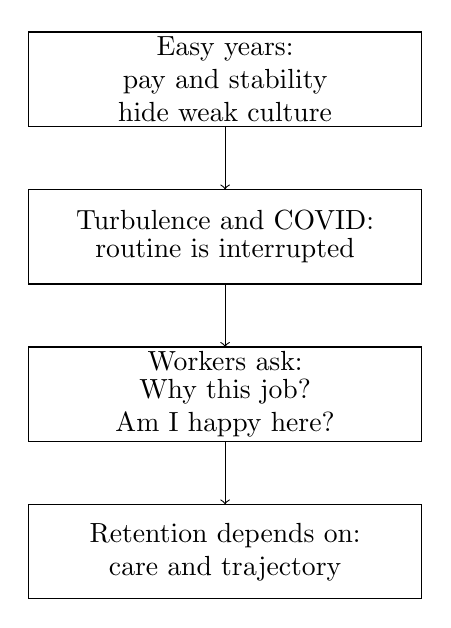
\begin{tikzpicture}[x=1cm,y=1cm]
\draw (0,0) rectangle (5,1.2);
\node at (2.5,0.6) {\shortstack{Easy years:\\pay and stability\\hide weak culture}};
\draw[->] (2.5,0)--(2.5,-0.8);
\draw (0,-2.0) rectangle (5,-0.8);
\node at (2.5,-1.4) {\shortstack{Turbulence and COVID:\\routine is interrupted}};
\draw[->] (2.5,-2.0)--(2.5,-2.8);
\draw (0,-4.0) rectangle (5,-2.8);
\node at (2.5,-3.4) {\shortstack{Workers ask:\\Why this job?\\Am I happy here?}};
\draw[->] (2.5,-4.0)--(2.5,-4.8);
\draw (0,-6.0) rectangle (5,-4.8);
\node at (2.5,-5.4) {\shortstack{Retention depends on:\\care and trajectory}};
\end{tikzpicture}
\end{figure}

\section{COVID and the Pause of Reflection}

The lecture now makes the mechanism concrete by naming COVID. The important point is not epidemiology as such. The important point is the pause: everyday motion stopped long enough for workers to ask what they were doing and why. Let us write the resulting question set as

\begin{align}
\mathcal{Q} = \{&
\text{Why do I do what I do?},\nonumber\\
&\text{Do I actually like my job?},\nonumber\\
&\text{Am I happy where I'm at?}\}.
\end{align}

The lecture's claim is that COVID increased the salience of this question set:

\begin{equation}
T_{\text{COVID}} \;\Rightarrow\; \mathcal{Q}.
\end{equation}

This is a useful place to be careful. The lecture does not offer a universal theorem of labor markets. It gives us a local but powerful mechanism: interruption produces reflection, and reflection changes the standard by which people evaluate work.

\section{Perks and False Explanations}

Once reflection begins, the lecture introduces a rejected model of retention. Many tech companies assumed that free food and similar benefits would be enough to keep people.

\begin{equation}
P \not\Rightarrow R .
\end{equation}

This does not mean perks are worthless in every conceivable situation. It means they are not sufficient to answer the questions that have now been brought to the surface. A perk can sweeten a job. It cannot by itself answer whether the company cares for the person or whether life is actually getting better.

The lecture's contrast is narrow and sharp:

\begin{itemize}
\item A perk-first model tries to retain people by adding convenience and surface benefits.
\item A care-growth model tries to retain people by improving how the person is treated and where that person's life is going.
\end{itemize}

\begin{proposition}
In the regime described by the lecture, a perk-first policy is insufficient as the central explanation of retention.
\end{proposition}

\begin{proof}
When turbulence rises, reevaluation rises. Reevaluation takes the form of questions about meaning, liking the work, and happiness in one's present situation. Perks do not directly answer this question set. The lecture's final answer is instead framed in terms of care and development. Hence a perk-first model cannot be the main retention mechanism once reevaluation has begun.
\end{proof}

\section{Care, Growth, and Retention}

The lecture resolves with two positive terms. People want to know that the company cares for them as persons, and they want room to grow, develop, and improve their life trajectory. As a compact mnemonic, let us define a transcript-based stay score:

\begin{equation}
S_{\text{stay}} = C + G .
\end{equation}

This is not a measured law. It is a concise way of preserving the speaker's final pairing. The operative implication is

\begin{equation}
C \uparrow \land G \uparrow \;\Rightarrow\; R \uparrow .
\end{equation}

If one wants a more general symbolic wrapper, one may write

\begin{equation}
\Pr(\text{stay}) = F(C,G,W,P;T),
\end{equation}

with the lecture strongly suggesting that, when turbulence is high, the decisive terms are \(C\) and \(G\), not \(P\).

\paragraph{Worked example.} To see the point cleanly, hold compensation fixed and compare two stylized firms during a turbulent period. Let Firm \(A\) be perk-heavy and Firm \(B\) be care-growth-heavy:

\begin{align}
A &: (C,G,P) = (1,1,3),\\
B &: (C,G,P) = (3,3,1).
\end{align}

Then the reconstructed score gives

\begin{align}
S_{\text{stay}}(A) &= C_A + G_A = 1+1 = 2,\\
S_{\text{stay}}(B) &= C_B + G_B = 3+3 = 6.
\end{align}

The point of the example is not to assign real numerical weights. It is to show the lecture's logic in compressed form. Once people are asking first-order questions about their lives, the firm with stronger care and clearer growth dominates the firm that merely offers better perks.

We can summarize the whole argument as a short chain:

\begin{align}
M \uparrow \land W \uparrow &\Rightarrow \text{retention can look strong even with weak culture},\\
T \uparrow &\Rightarrow E \uparrow,\\
T_{\text{COVID}} &\Rightarrow \mathcal{Q},\\
P \not\Rightarrow R,\\
C \uparrow \land G \uparrow &\Rightarrow R \uparrow .
\end{align}

This is the lecture's mathematical spine. It is modest, but it is sharp.

\section{Summary}

The lecture begins with a question about healthy work-life environment and answers it by way of a retention mechanism. First, repeated interviews reveal what workers actually complain about and seek. Second, easy years can mask unhealthy culture because pay and market stability keep retention artificially high. Third, turbulence and the COVID pause cause workers to reevaluate their lives and work. Fourth, perks do not solve that problem. The final operative principle is narrower and stronger: people stay when they are treated as persons and when they can see real growth in their trajectory.